\chapter{Open Sections B}
\label{ch:assignment2}

\begingroup\itshape Assignment 2 --- 20 points\endgroup



\bigskip


\begin{table}[h]
  \centering\small
  \caption{Plate thicknesses of the half section.}
  \label{tab:B1B2}
  \begin{tabular}{llcc}
        centre girder (half)      & $y=0$, $0<z<a$          & $2t_p$   & $2t_p$ \\
    bottom plating            & $0<y<2.5a$              & $3t_p$   & $3t_p$ \\
    bottom, bilge, side shell & $y>2.5a$ up to the deck & $2t_p$   & $2t_p$ \\
    inner bottom              & $0<y<4a$, $z=a$         & $2t_p$   & $3t_p$ \\
    longitudinal bulkhead     & $y=2.5a$, $0<z<5a$      & $2.5t_p$ & $t_p$  \\
    deck                      & $2.5a<y<4a$, $z=5a$     & $3t_p$   & $3t_p$ \\
    side girder               & $y=a$, $0<z<a$          & --       & $3t_p$ \\
    stringer deck             & $2.5a<y<4a$, $z=3a$     & --       & $t_p$  \\
  \end{tabular}
\end{table}

\section{Shear flow sketch for design B2}
\label{sec:a2-1}

\begin{figure}[H]
    \centering
    \begin{tikzpicture}[scale=1.3, >={Stealth[length=2.2mm,width=1.8mm]},
        cell/.style={circle, draw, inner sep=1pt, minimum size=4.6mm,
                     font=\footnotesize, fill=white},
        dim/.style={thin, {Latex[length=1.6mm,width=1.2mm]}-{Latex[length=1.6mm,width=1.2mm]}},
        ext/.style={very thin, gray}]

        % \flow{x}{y}{dx}{dy}{q}: arrow at (x,y) in direction (dx,dy), thickness ~ q,
        % plus the mirrored arrow in the port half
        \def\flow#1#2#3#4#5{%
            \pgfmathsetmacro{\lw}{max(0.4,#5/0.0331*2.4)}%
            \draw[->, red!75!black, line width=\lw pt]
                ({#1-0.2*(#3)},{#2-0.2*(#4)}) -- ({#1+0.2*(#3)},{#2+0.2*(#4)});
            \draw[->, red!75!black, line width=\lw pt]
                ({-(#1)-0.2*(#3)},{#2+0.2*(#4)}) -- ({-(#1)+0.2*(#3)},{#2-0.2*(#4)});
        }

        % ---------------- structure (starboard half, mirrored to port) ----------------
        \foreach \s in {1,-1}{
            \begin{scope}[xscale=\s]
                \draw[line width=1pt] (0,0) -- (3.5,0) arc (-90:0:0.5) -- (4,5) -- (2.5,5) -- (2.5,0);
                \draw[line width=1pt] (0,1) -- (4,1);   % inner bottom
                \draw[line width=1pt] (2.5,3) -- (4,3); % stringer deck
                \draw[line width=1pt] (1,0) -- (1,1);   % side girder
            \end{scope}
        }
        \draw[line width=2pt] (0,0) -- (0,1);           % centre girder
        \draw[dashed, gray] (0,-0.3) -- (0,5.3) node[above, black] {\small C.L.};

        % applied torque (counter-clockwise)
        \draw[->, thick] (0,3) ++(-30:0.6) arc (-30:210:0.6);
        \node at (0,3) {$M_t$};

        % ---------------- shear flow arrows ----------------
        % bottom shell
        \flow{0.5}{0}{1}{0}{0.0331}
        \flow{1.75}{0}{1}{0}{0.0312}
        \flow{3.0}{0}{1}{0}{0.0278}
        % inner bottom
        \flow{0.5}{1}{-1}{0}{0.0331}
        \flow{1.75}{1}{-1}{0}{0.0312}
        \flow{3.25}{1}{-1}{0}{0.0053}
        % girders in the double bottom
        \flow{1}{0.5}{0}{1}{0.0019}
        \flow{2.5}{0.5}{0}{1}{0.0034}
        % side shell
        \flow{4}{0.75}{0}{1}{0.0278}
        \flow{4}{2}{0}{1}{0.0225}
        \flow{4}{4}{0}{1}{0.0203}
        % inner side wall of the wing tanks
        \flow{2.5}{2}{0}{-1}{0.0225}
        \flow{2.5}{4}{0}{-1}{0.0203}
        % stringer deck and deck
        \flow{3.25}{3}{-1}{0}{0.0021}
        \flow{3.25}{5}{-1}{0}{0.0203}

        % ---------------- cell numbers ----------------
        \foreach \x/\y/\n in {0.5/0.5/1, 1.75/0.5/2, 2.8/0.5/3, 3.25/2/4, 3.25/4/5}{
            \node[cell] at (\x,\y) {\n};                          % starboard
            \node[cell, draw=gray, text=gray] at (-\x,\y) {\n};   % port (mirror)
        }

        % ---------------- bilge radius ----------------
        \fill (3.5,0.5) circle (0.8pt);
        \draw[thin, -{Latex[length=1.4mm,width=1mm]}] (3.5,0.5) -- ({3.5+0.5*cos(-45)},{0.5+0.5*sin(-45)});
        \node[font=\scriptsize, anchor=south] at (3.5,0.52) {$r=0.5a$};

        % ---------------- horizontal dimensions ----------------
        \foreach \x/\ytop in {0/-0.05, 1/-0.05, 2.5/-0.05, 4/0.4}{
            \draw[ext] (\x,\ytop) -- (\x,-0.65);
        }
        \draw[dim] (0,-0.5)   -- node[below, font=\small] {$a$}    (1,-0.5);
        \draw[dim] (1,-0.5)   -- node[below, font=\small] {$1.5a$} (2.5,-0.5);
        \draw[dim] (2.5,-0.5) -- node[below, font=\small] {$1.5a$} (4,-0.5);

        % ---------------- vertical dimensions ----------------
        \foreach \y/\xl in {0/3.55, 1/4.05, 3/4.05, 5/4.05}{
            \draw[ext] (\xl,\y) -- (5.0,\y);
        }
        \draw[dim] (4.9,0) -- node[right, font=\small] {$a$}  (4.9,1);
        \draw[dim] (4.9,1) -- node[right, font=\small] {$2a$} (4.9,3);
        \draw[dim] (4.9,3) -- node[right, font=\small] {$2a$} (4.9,5);
    \end{tikzpicture}
    \caption{Shear flow in design B2 for a counter-clockwise torque $M_t$. The arrow
    thickness is proportional to the magnitude of the shear flow. The cells are
    numbered 1--5 on both sides; the port cells (grey) are the mirror images of the
    starboard cells and carry the same shear flow. Because the two cells~1 on either
    side of the centre girder have equal flow, there is no net shear flow through
    the centre girder.}
    \label{fig:shearflow-B2}
\end{figure}

\newpage
\section{Shear flow per cell for design B2}
\label{sec:a2-2}

\questionbox{Calculate the shear flow per cell for design B2. Present all partial
answers. \textbf{(2 pts)}}

We use the multi-cell Bredt theory from the lectures. The $M_t$--$q$ relation (1st Bredt formula) and the $q$--$\theta$ relation (2nd Bredt formula, one for every cell) are

\begin{equation}
  M_t = 2\{\boldsymbol{\Omega}\}^T\{\mathbf{q}\}, \qquad
  [\mathbf{S}]\{\mathbf{q}\} = 2G\theta\{\boldsymbol{\Omega}\},
  \label{eq:B2_bredt}
\end{equation}

where all cells have the same twist rate $\theta$ (compatibility because the section
rotates as a rigid body). The contour matrix $[\mathbf{S}]$ has on the diagonal the
contour integral around cell $i$ and off the diagonal minus the integral over the
wall shared by cells $i$ and $j$:
\begin{equation}
  S_{ii} = \oint_i \frac{\mathrm{d}s}{t_p(s)}, \qquad
  S_{ij} = -\int_{ij} \frac{\mathrm{d}s}{t_p(s)} .
\end{equation}


\paragraph{Cell areas}
\begin{align*}
\Omega_1 &= a\cdot a = a^2 && \text{(double bottom, } 0<y<a\text{)}\\
\Omega_2 &= 1.5a\cdot a = 1.5a^2 && \text{(double bottom, } a<y<2.5a\text{)}\\
\Omega_3 &= 1.5a\cdot a - \left(0.5a\right)^2 + \tfrac{\pi}{4}(0.5a)^2
          = \left(1.25+\tfrac{\pi}{16}\right)a^2 = 1.446\,a^2
          && \text{(double bottom with bilge)}\\
\Omega_4 &= 1.5a\cdot 2a = 3a^2 && \text{(lower wing tank)}\\
\Omega_5 &= 1.5a\cdot 2a = 3a^2 && \text{(upper wing tank)}
\end{align*}
so
\begin{equation*}
  \{\boldsymbol{\Omega}\} = a^2\left\{1,\ 1.5,\ 1.25+\tfrac{\pi}{16},\ 3,\ 3\right\}^T .
\end{equation*}

\paragraph{Contour integrals per cell}
With the thicknesses of Table~\ref{tab:B1B2} (all terms in $a/t_p$):
\begin{align*}
\text{cell 1:}\quad S_{11} &= \underbrace{\tfrac{1}{3}}_{\text{bottom}}
   + \underbrace{\tfrac{1}{3}}_{\text{inner bottom}}
   + \underbrace{\tfrac{1}{3}}_{\text{side girder}} = 1,
   && S_{12} = -\tfrac{1}{3}\\
\text{cell 2:}\quad S_{22} &= \underbrace{\tfrac{1.5}{3}}_{\text{bottom}}
   + \underbrace{\tfrac{1.5}{3}}_{\text{inner bottom}}
   + \underbrace{\tfrac{1}{3}}_{\text{side girder}}
   + \underbrace{\tfrac{1}{1}}_{\text{bulkhead}} = \tfrac{7}{3},
   && S_{23} = -1\\
\text{cell 3:}\quad S_{33} &= \underbrace{\tfrac{1}{2}}_{\text{bottom}}
   + \underbrace{\tfrac{\pi/4}{2}}_{\text{bilge}}
   + \underbrace{\tfrac{0.5}{2}}_{\text{side}}
   + \underbrace{\tfrac{1.5}{3}}_{\text{inner bottom}}
   + \underbrace{\tfrac{1}{1}}_{\text{bulkhead}}
   = \tfrac{9}{4}+\tfrac{\pi}{8} = 2.643,
   && S_{34} = -\tfrac{1}{2}\\
\text{cell 4:}\quad S_{44} &= \underbrace{\tfrac{1.5}{3}}_{\text{inner bottom}}
   + \underbrace{\tfrac{2}{2}}_{\text{side}}
   + \underbrace{\tfrac{1.5}{1}}_{\text{stringer deck}}
   + \underbrace{\tfrac{2}{1}}_{\text{bulkhead}} = 5,
   && S_{45} = -1.5\\
\text{cell 5:}\quad S_{55} &= \underbrace{\tfrac{1.5}{1}}_{\text{stringer deck}}
   + \underbrace{\tfrac{2}{2}}_{\text{side}}
   + \underbrace{\tfrac{1.5}{3}}_{\text{deck}}
   + \underbrace{\tfrac{2}{1}}_{\text{bulkhead}} = 5
\end{align*}

\paragraph{Contour matrix and its inverse}
\begin{equation}
[\mathbf{S}] = \frac{a}{t_p}
\begin{bmatrix}
 1          & -\tfrac13 & 0                          & 0          & 0    \\
 -\tfrac13  & \tfrac73  & -1                         & 0          & 0    \\
 0          & -1        & \tfrac94+\tfrac{\pi}{8}    & -\tfrac12  & 0    \\
 0          & 0         & -\tfrac12                  & 5          & -1.5 \\
 0          & 0         & 0                          & -1.5       & 5
\end{bmatrix}
\ \rightarrow\
[\mathbf{S}]^{-1} = \frac{t_p}{a}
\begin{bmatrix}
 1.0605 & 0.1816 & 0.0702 & 0.0077 & 0.0023 \\
 0.1816 & 0.5447 & 0.2105 & 0.0231 & 0.0069 \\
 0.0702 & 0.2105 & 0.4678 & 0.0514 & 0.0154 \\
 0.0077 & 0.0231 & 0.0514 & 0.2254 & 0.0676 \\
 0.0023 & 0.0069 & 0.0154 & 0.0676 & 0.2203
\end{bmatrix}
\label{eq:B2_S}
\end{equation}

\paragraph{Solution}
Solving the $q$--$\theta$ relation gives
$\{\mathbf{q}\} = 2G\theta[\mathbf{S}]^{-1}\{\boldsymbol{\Omega}\}$ with
\begin{equation*}
  [\mathbf{S}]^{-1}\{\boldsymbol{\Omega}\}
  = a\,t_p\left\{1.4644,\ 1.3933,\ 1.2630,\ 0.9959,\ 0.8988\right\}^T,
  \qquad
  \{\boldsymbol{\Omega}\}^T[\mathbf{S}]^{-1}\{\boldsymbol{\Omega}\} = 11.065\,a^3t_p .
\end{equation*}
This is for the starboard half. The port half gives exactly the same contribution, so for the whole section $M_t = 2\cdot2\{\boldsymbol{\Omega}\}^T\{\mathbf{q}\}$
(half-section vectors). Filling in $\{\mathbf{q}\}$ gives
\begin{equation*}
  M_t = 8\,G\theta\,\{\boldsymbol{\Omega}\}^T[\mathbf{S}]^{-1}\{\boldsymbol{\Omega}\}
      = 88.52\,G\theta\,a^3t_p
  \quad\rightarrow\quad
  \theta = \frac{M_t}{88.52\,G\,a^3t_p} .
\end{equation*}
Substituting $\theta$ back into $\{\mathbf{q}\}$:
\begin{equation*}
  \{\mathbf{q}\} = \frac{M_t}{4}\cdot
  \frac{[\mathbf{S}]^{-1}\{\boldsymbol{\Omega}\}}
       {\{\boldsymbol{\Omega}\}^T[\mathbf{S}]^{-1}\{\boldsymbol{\Omega}\}}
\end{equation*}
\begin{equation}
  \{\mathbf{q}\} = G\theta\,a\,t_p
  \begin{Bmatrix} 2.929\\ 2.787\\ 2.526\\ 1.992\\ 1.798 \end{Bmatrix}
  = \frac{M_t}{a^2}
  \begin{Bmatrix} 0.0331\\ 0.0315\\ 0.0285\\ 0.0225\\ 0.0203 \end{Bmatrix} .
  \label{eq:B2_q}
\end{equation}


\finalanswer{
\[
q_1 = 0.0331\,\frac{M_t}{a^2},\quad
q_2 = 0.0315\,\frac{M_t}{a^2},\quad
q_3 = 0.0285\,\frac{M_t}{a^2},\quad
q_4 = 0.0225\,\frac{M_t}{a^2},\quad
q_5 = 0.0203\,\frac{M_t}{a^2},
\]
all counter-clockwise, with $\theta = M_t/(88.52\,G\,a^3t_p)$. The same flows act in
the mirrored port cells.}


\newpage
\section{Maximum shear stress for design B2}
\label{sec:a2-3}


\questionbox{Locate the position of maximum shear stress and its magnitude for design B2. \textbf{(2 pts)}}

The shear stress in a wall follows from the net shear flow in that wall and the local plate thickness:

\begin{equation}
    \tau(s_i) = \frac{q_i}{t_p(s_i)} .
    \label{eq:shear_stress}
\end{equation}

For an outer wall (or a wall facing the open hold) $q_i$ is the flow of that cell, for an internal wall it is the difference between the two cells. So the maximum does not have to be in the cell with the largest flow: a thin plate with a some smaller flow can give a higher stress. Table~\ref{tab:B2walls} gives all walls of the starboard half.

\begin{table}[h]
  \centering
  \caption{Net shear flow and shear stress per wall for design B2.}
  \label{tab:B2walls}
  \begin{tabular}{llcc}
    \toprule
    Wall & $t$ & $q_{net}$ [$M_t/a^2$] & $\tau = q_{net}/t$ [$M_t/(a^2t_p)$] \\
    \midrule
    Centre girder                           & $2t_p$ & $0$                       & $0$ \\
    Bottom and inner bottom, cell 1         & $3t_p$ & $q_1 = 0.0331$            & $0.0110$ \\
    Side girder                             & $3t_p$ & $q_1-q_2 = 0.0016$        & $0.0005$ \\
    Bottom and inner bottom, cell 2         & $3t_p$ & $q_2 = 0.0315$            & $0.0105$ \\
    Bulkhead in double bottom               & $t_p$  & $q_2-q_3 = 0.0029$        & $0.0029$ \\
    Bottom, bilge and side shell, cell 3    & $2t_p$ & $q_3 = 0.0285$            & $0.0143$ \\
    Inner bottom under wing tank            & $3t_p$ & $q_3-q_4 = 0.0060$        & $0.0020$ \\
    Side shell, cell 4                      & $2t_p$ & $q_4 = 0.0225$            & $0.0113$ \\
    \textbf{Bulkhead, cell 4}               & $\boldsymbol{t_p}$ & $\boldsymbol{q_4 = 0.0225}$ & $\boldsymbol{0.0225}$ \\
    Stringer deck                           & $t_p$  & $q_4-q_5 = 0.0022$        & $0.0022$ \\
    Side shell, cell 5                      & $2t_p$ & $q_5 = 0.0203$            & $0.0102$ \\
    Bulkhead, cell 5                        & $t_p$  & $q_5 = 0.0203$            & $0.0203$ \\
    Deck                                    & $3t_p$ & $q_5 = 0.0203$            & $0.0068$ \\
    \bottomrule
  \end{tabular}
\end{table}

The largest stress is in the longitudinal bulkhead of the lower wing tank (cell~4, $y=\pm2.5a$, between the inner bottom at $z=a$ and the stringer deck at $z=3a$). This plate is only $t_p$ thick and faces the open hold, so it carries the full flow $q_4$. The bulkhead of the upper wing tank (cell~5) comes second because $q_5$ is a bit smaller. The bottom shell has the largest flow ($q_1$), but it is $3t_p$ thick, so the stress there is only half as large.

\finalanswer{The maximum shear stress occurs in the longitudinal bulkhead of the lower wing tank (cell~4, $y=\pm2.5a$, $a<z<3a$), on both sides of the ship:

\[
  \tau_{max} = \frac{q_4}{t_p} = 0.0225\,\frac{M_t}{a^2t_p} = 1.99\,G\theta\,a .
\]}

\newpage

%=====================================================================
\section{Torsional stiffness and strength}
\label{sec:a2-4}

\questionbox{\begin{enumerate}[label=\alph*., leftmargin=*]
  \item Explain the difference between strength and stiffness. \textbf{(1 pt)}
  \item Analytically calculate the torsional stiffness $I_{p,B2}(a,t_p)$ for
        design B2 and compare this with the value
        $I_{p,B1}(a,t_p)\approx108.70\,a^3t_p$ of design B1. Discuss the origin
        of possible differences. \textbf{(2 pts)}
  \item Calculate the strength $M_{t,B2}(a,t_p,\tau_{max})$ for design B2 and
        compare this with the value
        $M_{t,B1}(a,t_p,\tau_{max})\approx75.50\,a^2t_p\tau_{max}$ of design B1.
        Discuss the origin of possible differences. \textbf{(2 pts)}
\end{enumerate}}

\begin{enumerate}[label=\alph*., leftmargin=*]
   \item \textbf{Strength vs.\ stiffness.}
  Stiffness says how much something deforms under a load, strength says how much load it can take before it breaks or yields. They sound similar, but they are really two different things.

  A good example of something that is stiff but not strong is glass. A glass plate hardly bends when you push on it (its $E$ of about 70\,GPa is similar to aluminium), but it breaks suddenly at a fairly low stress because it is brittle and small surface cracks grow very fast. The other way around, a nylon fishing
  line is strong but not stiff: it can hold a heavy fish without breaking, but it stretches a lot before that happens.

  For torsion it works the same way. The stiffness follows from the
  
  $M_t$--$\theta$ relation
  \begin{equation}
    M_t = G\,\theta\,I_p ,
  \end{equation}
  
  so $GI_p$ tells you how much torque is needed to twist the section. $G$ comes from the material and $I_p$ from the shape of the whole section. The strength is the torque at which the shear stress $\tau = q/t_p$ reaches $\tau_{max}$ somewhere in the section. That means strength is decided by one weak spot, usually a thin plate with a large shear flow, while stiffness depends on the whole section.



  \emph{Strength} is the maximum load the section can carry before the stress
  somewhere reaches the allowable value $\tau_{max}$. For torsion we look at the
  shear stress $\tau(s_i) = q_i/t_p(s_i)$ and find the location where it is highest.
  The strength is the torque $M_t$ for which $\tau$ at that location equals
  $\tau_{max}$. So strength is decided by one critical point in the section,
  usually a thin plate that carries a large shear flow.

  Because of this, a design change can affect the two very differently. An example
  from the lectures is the open and closed thin walled circular section: closing
  the section makes it a factor $3(r/t_p)^2$ stiffer, but the maximum stress also
  depends on where the thinnest, most loaded plate is. A structure can be stiff
  but not strong (a thin plate somewhere is overloaded), or strong but not stiff
  (low stresses, but still a lot of twist).

  \item \textbf{Torsional stiffness of B2.}
  From the $M_t$--$\theta$ relation of the lectures:
  \begin{equation}
    I_p = 4\{\boldsymbol{\Omega}\}^T[\mathbf{S}]^{-1}\{\boldsymbol{\Omega}\} .
  \end{equation}
  Using the half-section vectors of Section~\ref{sec:a2-2} and counting both
  halves:
  \begin{equation}
    I_{p,B2} = 2\cdot4\{\boldsymbol{\Omega}\}^T[\mathbf{S}]^{-1}\{\boldsymbol{\Omega}\}
             = 8\cdot11.065\,a^3t_p = 88.52\,a^3t_p .
  \end{equation}
  Compared to B1:
  \begin{equation}
    \frac{I_{p,B2}}{I_{p,B1}} = \frac{88.52}{108.70} = 0.81 ,
  \end{equation}
  so B2 is about 19\,\% \emph{less} stiff, even though it uses the same amount of material and has one extra stringer and girder.

  The reason is where the material is placed. In Bredt theory the stiffness is mainly decided by the enclosed area and by $\oint\mathrm{d}s/t$ along the outer contour of the closed part (the walls that carry the full cell flow). The outer parts is the same for both designs, so $\{\boldsymbol{\Omega}\}$ hardly changes. The new side girder and stringer deck are internal walls: they only carry the difference between two cell flows ($q_1-q_2$ and $q_4-q_5$, both below $0.0025\,M_t/a^2$), so they add almost nothing to $I_p$. The material for these walls is taken from the longitudinal bulkhead, which goes from $2.5t_p$ to $t_p$. That bulkhead is part of the outer contour of the closed structure (it faces the open hold), so its $L/t$ term goes up from $5a/(2.5t_p) = 2\,a/t_p$ to $5a/t_p$. The thicker inner bottom in B2 ($3t_p$ instead of $2t_p$) helps a bit, but not enough to compensate.

  \item \textbf{Strength of B2.}
  The shear stress reaches $\tau_{max}$ first in the bulkhead of cell~4
  (Section~\ref{sec:a2-3}), with $t_p(s) = t_p$. Using
  $\tau(s_i) = q_i/t_p(s_i)$ and the expression for $\{\mathbf{q}\}$ from
  Section~\ref{sec:a2-2}:
  \begin{equation}
    \tau_{max} = \frac{q_4}{t_p}
    = \frac{M_t}{4\,t_p}\cdot
      \frac{\big([\mathbf{S}]^{-1}\{\boldsymbol{\Omega}\}\big)_4}
           {\{\boldsymbol{\Omega}\}^T[\mathbf{S}]^{-1}\{\boldsymbol{\Omega}\}}
    = \frac{M_t}{4\,t_p}\cdot\frac{0.9959\,a\,t_p}{11.065\,a^3t_p}
    = 0.0225\,\frac{M_t}{a^2t_p} .
  \end{equation}
  Setting $\tau = \tau_{max}$ and solving for $M_t$:
  \begin{equation}
    M_{t,B2} = \frac{4\,t_p\,\{\boldsymbol{\Omega}\}^T[\mathbf{S}]^{-1}\{\boldsymbol{\Omega}\}}
                    {\big([\mathbf{S}]^{-1}\{\boldsymbol{\Omega}\}\big)_4}\,\tau_{max}
             = \frac{4\cdot11.065}{0.9959}\,a^2t_p\,\tau_{max}
             = 44.44\,a^2t_p\,\tau_{max} .
  \end{equation}
  Compared to B1:
  \begin{equation}
    \frac{M_{t,B2}}{M_{t,B1}} = \frac{44.44}{75.50} = 0.59 ,
  \end{equation}
  so B2 can carry about 41\,\% less torque.

  In B1 the maximum stress is in the $2t_p$ side shell of the wing tank. In B2 it moves to the bulkhead of cell~4, which is only $t_p$ thick but carries exactly the same flow $q_4$ as the side shell next to it. The flow there is actually a bit lower than in B1 ($0.0225$ vs.\ $0.0265\,M_t/a^2$), because the wing tank is now split into two cells. But since the plate is half as thick, the stress still goes up by a factor of about 1.7. That is why the strength drops much more (41\,\%) than the stiffness (19\,\%). The extra side girder and stringer deck may be useful for other things (bending, buckling of the plating, local loads from the tanks), but for torsion they make the section worse.
\end{enumerate}

\finalanswer{
\begin{enumerate}[label=\alph*., leftmargin=*]
  \item Stiffness ($GI_p$, from $M_t = G\theta I_p$) is the resistance against
        twisting of the whole section; strength is the maximum torque before
        $\tau = q/t_p$ reaches $\tau_{max}$ in the most critical point.
  \item $I_{p,B2} = 8\{\boldsymbol{\Omega}\}^T[\mathbf{S}]^{-1}\{\boldsymbol{\Omega}\}
        = 88.52\,a^3t_p$, which is 19\,\% lower than $I_{p,B1} = 108.70\,a^3t_p$,
        because material is moved from the outer contour (bulkhead $2.5t_p\to t_p$)
        to internal walls that carry almost no net shear flow.
  \item $M_{t,B2} = 44.44\,a^2t_p\,\tau_{max}$, which is 41\,\% lower than
        $M_{t,B1} = 75.50\,a^2t_p\,\tau_{max}$, because the maximum stress now occurs
        in the thin ($t_p$) bulkhead of the lower wing tank.
\end{enumerate}}


\newpage
%=====================================================================
\newpage
\section{Sectorial coordinate and sectorial area moment}
\label{sec:a2-5}

\questionbox{Calculate and plot, for this U-shaped structure, the sectorial
coordinate distribution $\omega(s)$ as well as the sectorial area moment
$S_\omega(s)$ for design BU, in order to show the cross-sectional warping
displacement and shear stress distribution. Sketch the distributions in the
U-shaped section. \textbf{(3 pts)}}

\subsection{Pole coordinates}

The pole must be placed in the twist centre, because only then does $\omega$ describe pure warping without a contribution from bending. The twist centre is at the same place as the shear centre S, the point through which a shear force causes bending without twisting. Because of the symmetry of the section, S lies on the centre line. Its distance $e$ below the bottom plate comes from moment equilibrium of the shear flows due to a horizontal shear force $F_y$ acting through S. The geometry, contour points and pole are shown in Figure~\ref{fig:BU_section}.

\begin{figure}[h]
    \centering
    \begin{tikzpicture}[scale=0.75, >={Stealth[length=2.2mm,width=1.8mm]},
        pt/.style={circle, draw, inner sep=1pt, minimum size=4.6mm,
                   font=\footnotesize, fill=white},
        dim/.style={thin, {Latex[length=1.6mm,width=1.2mm]}-{Latex[length=1.6mm,width=1.2mm]}},
        ext/.style={very thin, gray}]

        \pgfmathsetmacro{\ee}{1.672}   % e = 1.672a

        % ---------------- structure (line width ~ plate thickness) ----------------
        \draw[line width=1.4pt] (-4,5) -- (-4,0);                 % port side,  t_sp
        \draw[line width=1.4pt] ( 4,5) -- ( 4,0);                 % stb side,   t_sp
        \draw[line width=2.6pt, line cap=rect] (-4,0) -- (4,0);   % bottom,     t_bp
        \draw[dashed, gray] (0,-2.0) -- (0,5.4) node[above, black] {\small C.L.};

        % ---------------- contour points ----------------
        \node[pt] at (-4, 5.55)     {1};
        \node[pt] at (-4.55,-0.55)  {2};
        \node[pt] at ( 0.5, 0.5)    {3};
        \node[pt] at ( 4.55,-0.55)  {4};
        \node[pt] at ( 4, 5.55)     {5};

        % ---------------- z = e (omega = 0 on the sides) ----------------
        \foreach \s in {-1,1} \draw[thin] ({\s*3.8},\ee) -- ({\s*4.2},\ee);
        \node[font=\scriptsize, right] at (-3.8,\ee) {$z=e$};

        % ---------------- shear centre / pole ----------------
        \fill[red!70!black] (0,-\ee) circle (2.2pt);
        \node[right, font=\small, red!70!black] at (0.1,-\ee) {S ($=$ CT)};

        % ---------------- thickness labels ----------------
        \node[left,  font=\small] at (-4.1,2.8) {$t_{sp}$};
        \node[below, font=\small] at (-2,-0.1)  {$t_{bp}$};

        % ---------------- dimension e ----------------
        \draw[ext] (0,-\ee) -- (-0.85,-\ee);
        \draw[dim] (-0.7,0) -- node[left, font=\small] {$e$} (-0.7,-\ee);

        % ---------------- dimension A ----------------
        \foreach \x in {-4,4} \draw[ext] (\x,-0.15) -- (\x,-2.55);
        \draw[dim] (-4,-2.4) -- node[below, font=\small] {$A = 8a$} (4,-2.4);

        % ---------------- dimension B ----------------
        \foreach \y in {0,5} \draw[ext] (4.15,\y) -- (5.15,\y);
        \draw[dim] (5.0,0) -- node[right, font=\small] {$B = 5a$} (5.0,5);

        % ---------------- coordinate system ----------------
        \draw[->] (-6.2,-1.8) -- (-5.4,-1.8) node[right, font=\small] {$y$};
        \draw[->] (-6.2,-1.8) -- (-6.2,-1.0) node[above, font=\small] {$z$};
    \end{tikzpicture}
    \caption{U-shaped section of design BU ($A=8a$, $B=5a$, $t_{sp}=3.5t_p$,
             $t_{bp}=6.5t_p$) with contour points 1--5 and shear (twist) centre S at a
             distance $e=1.672a$ below the bottom plate.}
    \label{fig:BU_section}
\end{figure}

The shear flow due to $F_y$ follows from
\begin{equation}
    q(s) = \frac{F_y\,S_z(s)}{I_{zz}},
\end{equation}
where $S_z(s)$ is the first moment of area of the part between the free edge and the
considered point, and
\begin{equation}
    I_{zz} = \frac{t_{bp}A^3}{12} + 2Bt_{sp}\left(\frac{A}{2}\right)^2
    = \left(\frac{6.5\cdot8^3}{12} + 2\cdot5\cdot3.5\cdot4^2\right)a^3t_p
    = (277.3 + 560)\,a^3t_p = 837.3\,a^3t_p .
\end{equation}
Because the entire side shell lies at $|y| = A/2$, the first moment of area of a side
shell, measured from the free edge down to height $z$, is
$S_z = \frac{A}{2}\,t_{sp}(B-z)$. The shear flow in a side shell is therefore
\begin{equation}
    q(z) = F_y\,\frac{\frac{A}{2}\,t_{sp}\,(B-z)}{I_{zz}},
\end{equation}
giving a vertical resultant per side shell
\begin{equation}
    V = \int_0^B q(z)\,\mathrm{d}z = F_y\,\frac{\frac{A}{2}\,t_{sp}\,\frac{B^2}{2}}{I_{zz}} .
\end{equation}
The resultants in the two side shells act in opposite directions and form a couple $V \cdot A$. The resultant of the shear flow in the bottom plate acts along the bottom plate itself and has no moment about point 3. The couple must therefore be balanced by
$F_y$ acting at a distance $e$ below the bottom:
\begin{equation}
    F_y\,e = V A \quad\Rightarrow\quad
    e = \frac{3B^2t_{sp}}{A\,t_{bp} + 6B\,t_{sp}} = \frac{262.5}{157}\,a = 1.672\,a .
\end{equation}
The pole coordinates are therefore $(y,z)_S = (0,\,-1.672a)$.

\subsection{Sectorial coordinate}

With free warping torsion, the cross-section warps out of its plane. The warping displacement is written as the product of an amplitude and a distribution:
\begin{equation}
    \underbrace{u(s)}_{\substack{\text{Warping}\\ \text{displacement}}}
    = \underbrace{\theta}_{\substack{\text{Warping amplitude}\\ \text{(twist rate)}}}
    \cdot \underbrace{\omega(s)}_{\substack{\text{Warping distribution}\\ \text{(\textbf{sectorial coordinate})}}}
\end{equation}
with the sectorial coordinate
\begin{equation}
    \omega(s) = -\int_s \rho(s)\,\mathrm{d}s + C ,
\end{equation}
where $\rho$ is the perpendicular distance from the pole S to the tangent of the
contour, taken positive when the radius vector from S rotates counterclockwise
along $s$. The integration starts at point 3, where the contour intersects the
symmetry axis; there $\omega = 0$, so $C = 0$.

The contour is split into parts. Each part gets its own local coordinate $s$, which
starts at $s=0$ at the beginning of that part. The constant $C$ of a part is the
value of $\omega$ at the end of the previous part, so that $\omega$ stays continuous
at the corners.

\begin{figure}[h]
  \centering
  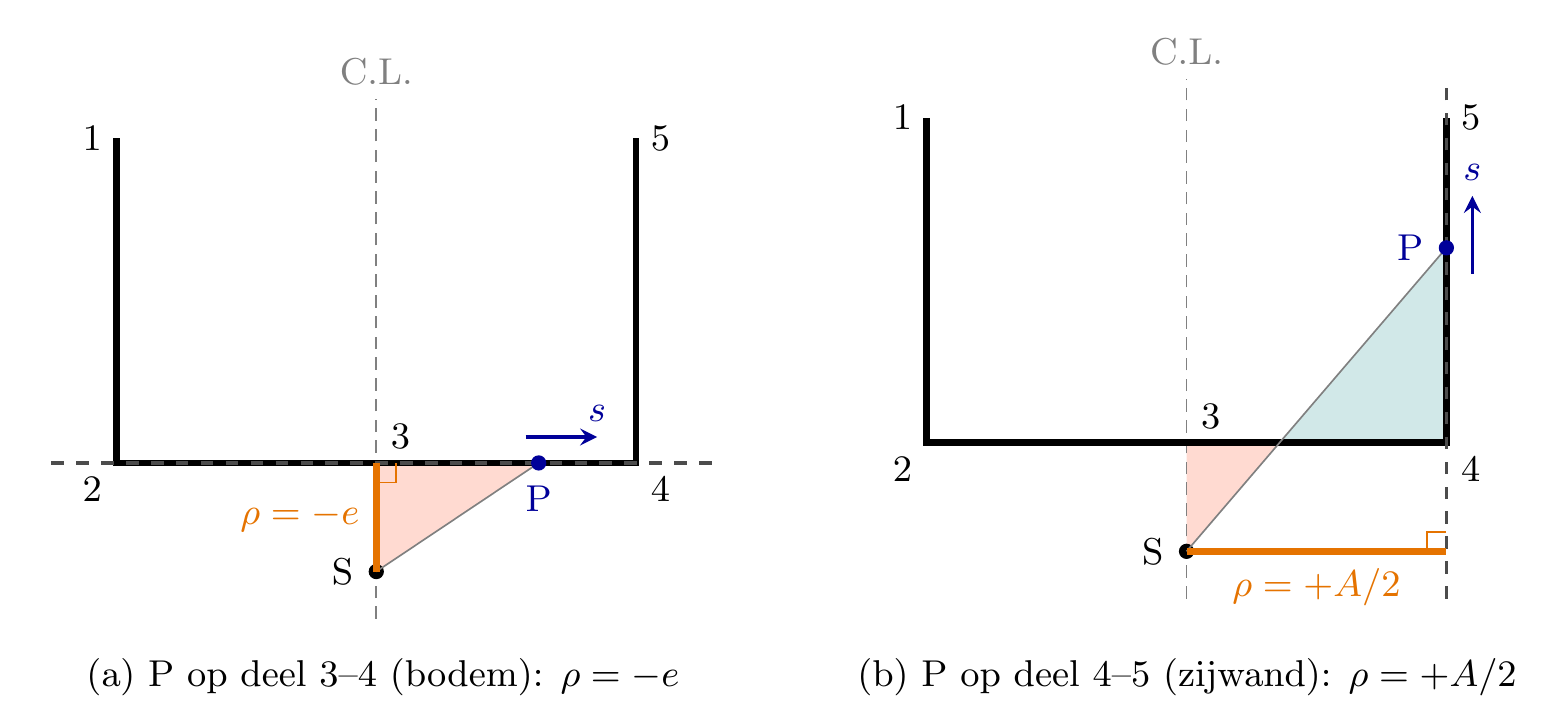
\includegraphics[width=0.9\textwidth]{figures/rho_figuur}
  \caption{Definition of $\rho$ for the U-shaped section BU. Left: P on the bottom
    plate (part 3--4), $\rho=-e$. Right: P on the side shell (part 4--5),
    $\rho=+A/2$.}
  \label{fig:rho}
\end{figure}

\newpage

\paragraph{Part 3--2 (bottom plate, port half).}
The bottom plate lies at a distance $e$ above the pole, so $|\rho| = e$. Walking from
point 3 to point 2 (in negative $y$-direction), the radius vector from S turns
counter-clockwise, so $\rho = +e$. With $C=0$ this gives
\begin{equation}
    \omega_{32}(s) = -\int_0^s e\,\mathrm{d}s = -e\,s ,
    \qquad 0 \le s \le \tfrac{A}{2},
\end{equation}
so in point 2
\begin{equation}
    \omega_2 = -e\,\frac{A}{2} = -1.672 \cdot 4\,a^2 = -6.69\,a^2 .
\end{equation}

\paragraph{Part 2--1 (port side shell).}
The side shell is vertical and lies at a distance $A/2$ from the pole, so
$|\rho| = A/2$. Walking upwards from point 2 to point 1, the radius vector turns
clockwise, so $\rho = -A/2$. The integration now starts at $\omega_2$, so
$C = -eA/2$:
\begin{equation}
    \omega_{21}(s) = -\int_0^s \left(-\frac{A}{2}\right)\mathrm{d}s - e\,\frac{A}{2}
                   = \frac{A}{2}\,(s-e) ,
    \qquad 0 \le s \le B .
\end{equation}
Here $s$ is equal to the height $z$ above the bottom. The sectorial coordinate is
zero at $s = z = e$ and reaches its maximum at the free edge:
\begin{equation}
    \omega_1 = \frac{A}{2}\,(B-e) = 4 \cdot 3.328\,a^2 = 13.31\,a^2 .
\end{equation}

\paragraph{Starboard half (3--4--5).}
Because the section is symmetric about the centre line, $\omega$ is antisymmetric:
the starboard half has the same magnitudes with the opposite sign,
\begin{equation}
    \omega_{34}(s) = e\,s , \qquad
    \omega_{45}(s) = -\frac{A}{2}\,(s-e) ,
\end{equation}
so $\omega_4 = +6.69\,a^2$ and $\omega_5 = -13.31\,a^2$.

\paragraph{Normalisation and check.}
The constant $C=0$ in point 3 is only correct if free warping does not create a net normal force, so $\int_A \omega\,\mathrm{d}A = 0$ must hold. Since $\omega$ is antisymmetric about the centre line, the contributions of the port and starboard halves cancel each other out, so this condition is satisfied.

As a check on the pole position, free warping should also not create a bending
moment, so $\int_A \omega\,y\,\mathrm{d}A = 0$. With $\omega_{bottom} = e\,y$ and
$y = \pm A/2$ on the side shells:
\begin{equation}
    \int_A \omega\,y\,\mathrm{d}A
    = e\,\frac{t_{bp}A^3}{12} - \frac{A^2}{2}\,t_{sp}\left(\frac{B^2}{2} - eB\right)
    = 463.7 - 463.7 = 0\ \ [a^5t_p],
\end{equation}
which confirms that $e = 1.672a$ is the correct pole position.

\subsection{Sectorial area moment}

When warping is blocked, a warping shear flow develops in the cross-section. Its distribution over the contour is given by the sectorial area moment
\begin{equation}
    S_\omega(s) = -t\int_s \omega(s)\,\mathrm{d}s + C .
\end{equation}
The integration starts at a free edge, because no shear flow can leave the section there. Starting at point 1 therefore gives $S_\omega = 0$ and $C = 0$. Again every part gets its own local $s$, and $C$ is the value at the end of the previous part.

\paragraph{Part 1--2 (port side shell, downwards).}
Now $s$ runs downwards from point 1, so the height is $z = B - s$ and the sectorial
coordinate in this local coordinate is
\begin{equation}
    \omega_{12}(s) = \frac{A}{2}\,(B - s - e) .
\end{equation}
Integrating gives
\begin{equation}
    S_{\omega,12}(s) = -t_{sp}\int_0^s \frac{A}{2}\,(B - e - s)\,\mathrm{d}s
    = t_{sp}\,\frac{A}{2}\left[\frac{s^2}{2} - (B-e)\,s\right],
    \qquad 0 \le s \le B ,
\end{equation}
with $t_{sp}\,A/2 = 14\,a\,t_p$. Since $\mathrm{d}S_\omega/\mathrm{d}s = -t\,\omega$,
the extremum lies where $\omega = 0$, so at $s = B-e$ (height $z=e$):
\begin{equation}
    S_{\omega,\max} = -t_{sp}\,\frac{A}{2}\,\frac{(B-e)^2}{2}
    = -14 \cdot 5.54\,a^3t_p = -77.5\,a^3t_p .
\end{equation}
In point 2 ($s = B$):
\begin{equation}
    S_{\omega,2} = t_{sp}\,\frac{A}{2}\left(eB - \frac{B^2}{2}\right)
    = 14\,(8.36 - 12.5)\,a^3t_p = -58.0\,a^3t_p .
\end{equation}

\paragraph{Part 2--3 (bottom plate, towards the centre).}
Now $s$ runs from point 2 to point 3, so
\begin{equation}
    \omega_{23}(s) = -e\,\frac{A}{2} + e\,s .
\end{equation}
The integration starts at $S_{\omega,2}$:
\begin{equation}
    S_{\omega,23}(s) = -t_{bp}\int_0^s \left(-e\,\frac{A}{2} + e\,s\right)\mathrm{d}s
                       + S_{\omega,2}
    = t_{bp}\,e\left[\frac{A}{2}\,s - \frac{s^2}{2}\right] + S_{\omega,2},
    \qquad 0 \le s \le \tfrac{A}{2}.
\end{equation}
In point 3 ($s = A/2$), where $\omega = 0$ and $S_\omega$ has its second extremum:
\begin{equation}
    S_{\omega,3} = t_{bp}\,e\,\frac{A^2}{8} + S_{\omega,2}
    = (86.9 - 58.0)\,a^3t_p = +29.0\,a^3t_p .
\end{equation}

\paragraph{Starboard half (3--4--5).}
Because $\omega$ is antisymmetric, $S_\omega$ is symmetric about the centre line. So
$S_{\omega,4} = -58.0\,a^3t_p$, the extremum in the starboard side shell is again
$-77.5\,a^3t_p$ at $z=e$, and at the free edge
\begin{equation}
    S_{\omega,5} = -\int_A \omega\,\mathrm{d}A = 0 ,
\end{equation}
as it should be at a free edge.

\newpage
\subsection{Distributions}

Both distributions are sketched in the U-shaped section in Figure~\ref{fig:BU_distributions}, and the values in the characteristic points are listed in Table~\ref{tab:BU_values}. The sectorial coordinate is linear along each part, the sectorial area moment is quadratic along each part.

\begin{figure}[h]
    \centering
    \begin{tikzpicture}[scale=0.45,
        pos/.style={fill=red!25, draw=red!70!black, thin},
        neg/.style={fill=blue!20, draw=blue!70!black, thin},
        val/.style={font=\scriptsize}]

        \pgfmathsetmacro{\ee}{1.672}

        % ================= sectorial coordinate omega =================
        \begin{scope}
            \filldraw[pos] (-4,5) -- (-5.6,5) -- (-4,\ee) -- cycle;   % port, upper
            \filldraw[neg] (-4,\ee) -- (-3.2,0) -- (-4,0) -- cycle;   % port, lower
            \filldraw[neg] (4,5) -- (2.4,5) -- (4,\ee) -- cycle;      % stb, upper
            \filldraw[pos] (4,\ee) -- (4.8,0) -- (4,0) -- cycle;      % stb, lower
            \filldraw[neg] (-4,0) -- (-4,0.8) -- (0,0) -- cycle;      % bottom, port
            \filldraw[pos] (0,0) -- (4,-0.8) -- (4,0) -- cycle;       % bottom, stb

            \draw[line width=1.2pt] (-4,5) -- (-4,0) -- (4,0) -- (4,5);
            \draw[dashed, gray] (0,-1.2) -- (0,5.6);

            \node[val, above] at (-5.6,5) {$+13.31$};
            \node[val, above] at (2.4,5)  {$-13.31$};
            \node[val, right] at (-3.1,1.1) {$-6.69$};
            \node[val, right] at (4.8,-0.4) {$+6.69$};
            \node at (0,-2.2) {$\omega$ [$a^2$]};
        \end{scope}

        % ================= sectorial area moment S_omega =================
        \begin{scope}[shift={(13,0)}]
            % port side shell (all negative, plotted inside)
            \filldraw[neg] plot[domain=0:5, samples=40]
                ({-4-0.02*14*(1.672*(5-\x)-(25-(\x)*(\x))/2)},{\x})
                -- (-4,5) -- (-4,0) -- cycle;
            % starboard side shell (mirror)
            \filldraw[neg] plot[domain=0:5, samples=40]
                ({4+0.02*14*(1.672*(5-\x)-(25-(\x)*(\x))/2)},{\x})
                -- (4,5) -- (4,0) -- cycle;
            % bottom plate: negative near the corners, positive in the middle
            \filldraw[neg] plot[domain=-4:-2.308, samples=20]
                ({\x},{-0.02*(-57.96-5.434*((\x)*(\x)-16))})
                -- (-2.308,0) -- (-4,0) -- cycle;
            \filldraw[neg] plot[domain=2.308:4, samples=20]
                ({\x},{-0.02*(-57.96-5.434*((\x)*(\x)-16))})
                -- (4,0) -- (2.308,0) -- cycle;
            \filldraw[pos] plot[domain=-2.308:2.308, samples=30]
                ({\x},{-0.02*(-57.96-5.434*((\x)*(\x)-16))}) -- cycle;

            \draw[line width=1.2pt] (-4,5) -- (-4,0) -- (4,0) -- (4,5);
            \draw[dashed, gray] (0,-1.2) -- (0,5.6);

            \node[val, above] at (-4,5.1) {$0$};
            \node[val, above] at (4,5.1)  {$0$};
            \node[val, right] at (-2.4,\ee) {$-77.5$};
            \node[val, left]  at (2.4,\ee)  {$-77.5$};
            \node[val, below left]  at (-4,-0.1) {$-58.0$};
            \node[val, below right] at (4,-0.1)  {$-58.0$};
            \node[val, below] at (0,-0.6) {$+29.0$};
            \node at (0,-2.2) {$S_\omega$ [$a^3t_p$]};
        \end{scope}
    \end{tikzpicture}
    \caption{Sectorial coordinate $\omega$ (left) and sectorial area moment $S_\omega$
             (right) along the contour of design BU. Positive values are plotted on
             the outside of the section, negative values on the inside.}
    \label{fig:BU_distributions}
\end{figure}

\begin{table}[h]
    \centering
    \caption{Sectorial coordinate and sectorial area moment in the characteristic
             points of design BU.}
    \label{tab:BU_values}
    \begin{tabular}{llrr}
        \hline
        Point & Location & $\omega$ [$a^2$] & $S_\omega$ [$a^3t_p$] \\
        \hline
        1 & top of port side       & $+13.31$ & $0$     \\
          & port side, $z=e$       & $0$      & $-77.5$ \\
        2 & port corner            & $-6.69$  & $-58.0$ \\
        3 & bottom centre          & $0$      & $+29.0$ \\
        4 & starboard corner       & $+6.69$  & $-58.0$ \\
          & starboard side, $z=e$  & $0$      & $-77.5$ \\
        5 & top of starboard side  & $-13.31$ & $0$     \\
        \hline
    \end{tabular}
\end{table}

\paragraph{Warping displacement.}
Since $u = \theta\,\omega$, the shape of $\omega$ directly shows how the section warps. The tops of the side shells warp the most, and in opposite directions: one moves forward while the other moves aft. The bottom corners warp a bit in the opposite direction of the top of the same side shell. Point 3 and the points at $z=e$ on the side shells do not warp at all.

\paragraph{Warping shear stress.}
The warping shear stress is proportional to $S_\omega/t$. It is zero at the free edges and largest in the side shells at $z=e$, where $|S_\omega|/t_{sp} = 77.5/3.5 = 22.1\,a^3$. In the bottom plate it is much lower: $58.0/6.5 = 8.9\,a^3$ in the corners and $29.0/6.5 = 4.5\,a^3$ in the bottom centre, because $|S_\omega|$ is smaller there and the bottom plate is almost twice as thick. So the side shells carry most of the warping shear stress.

\begin{figure}[H]
  \centering
  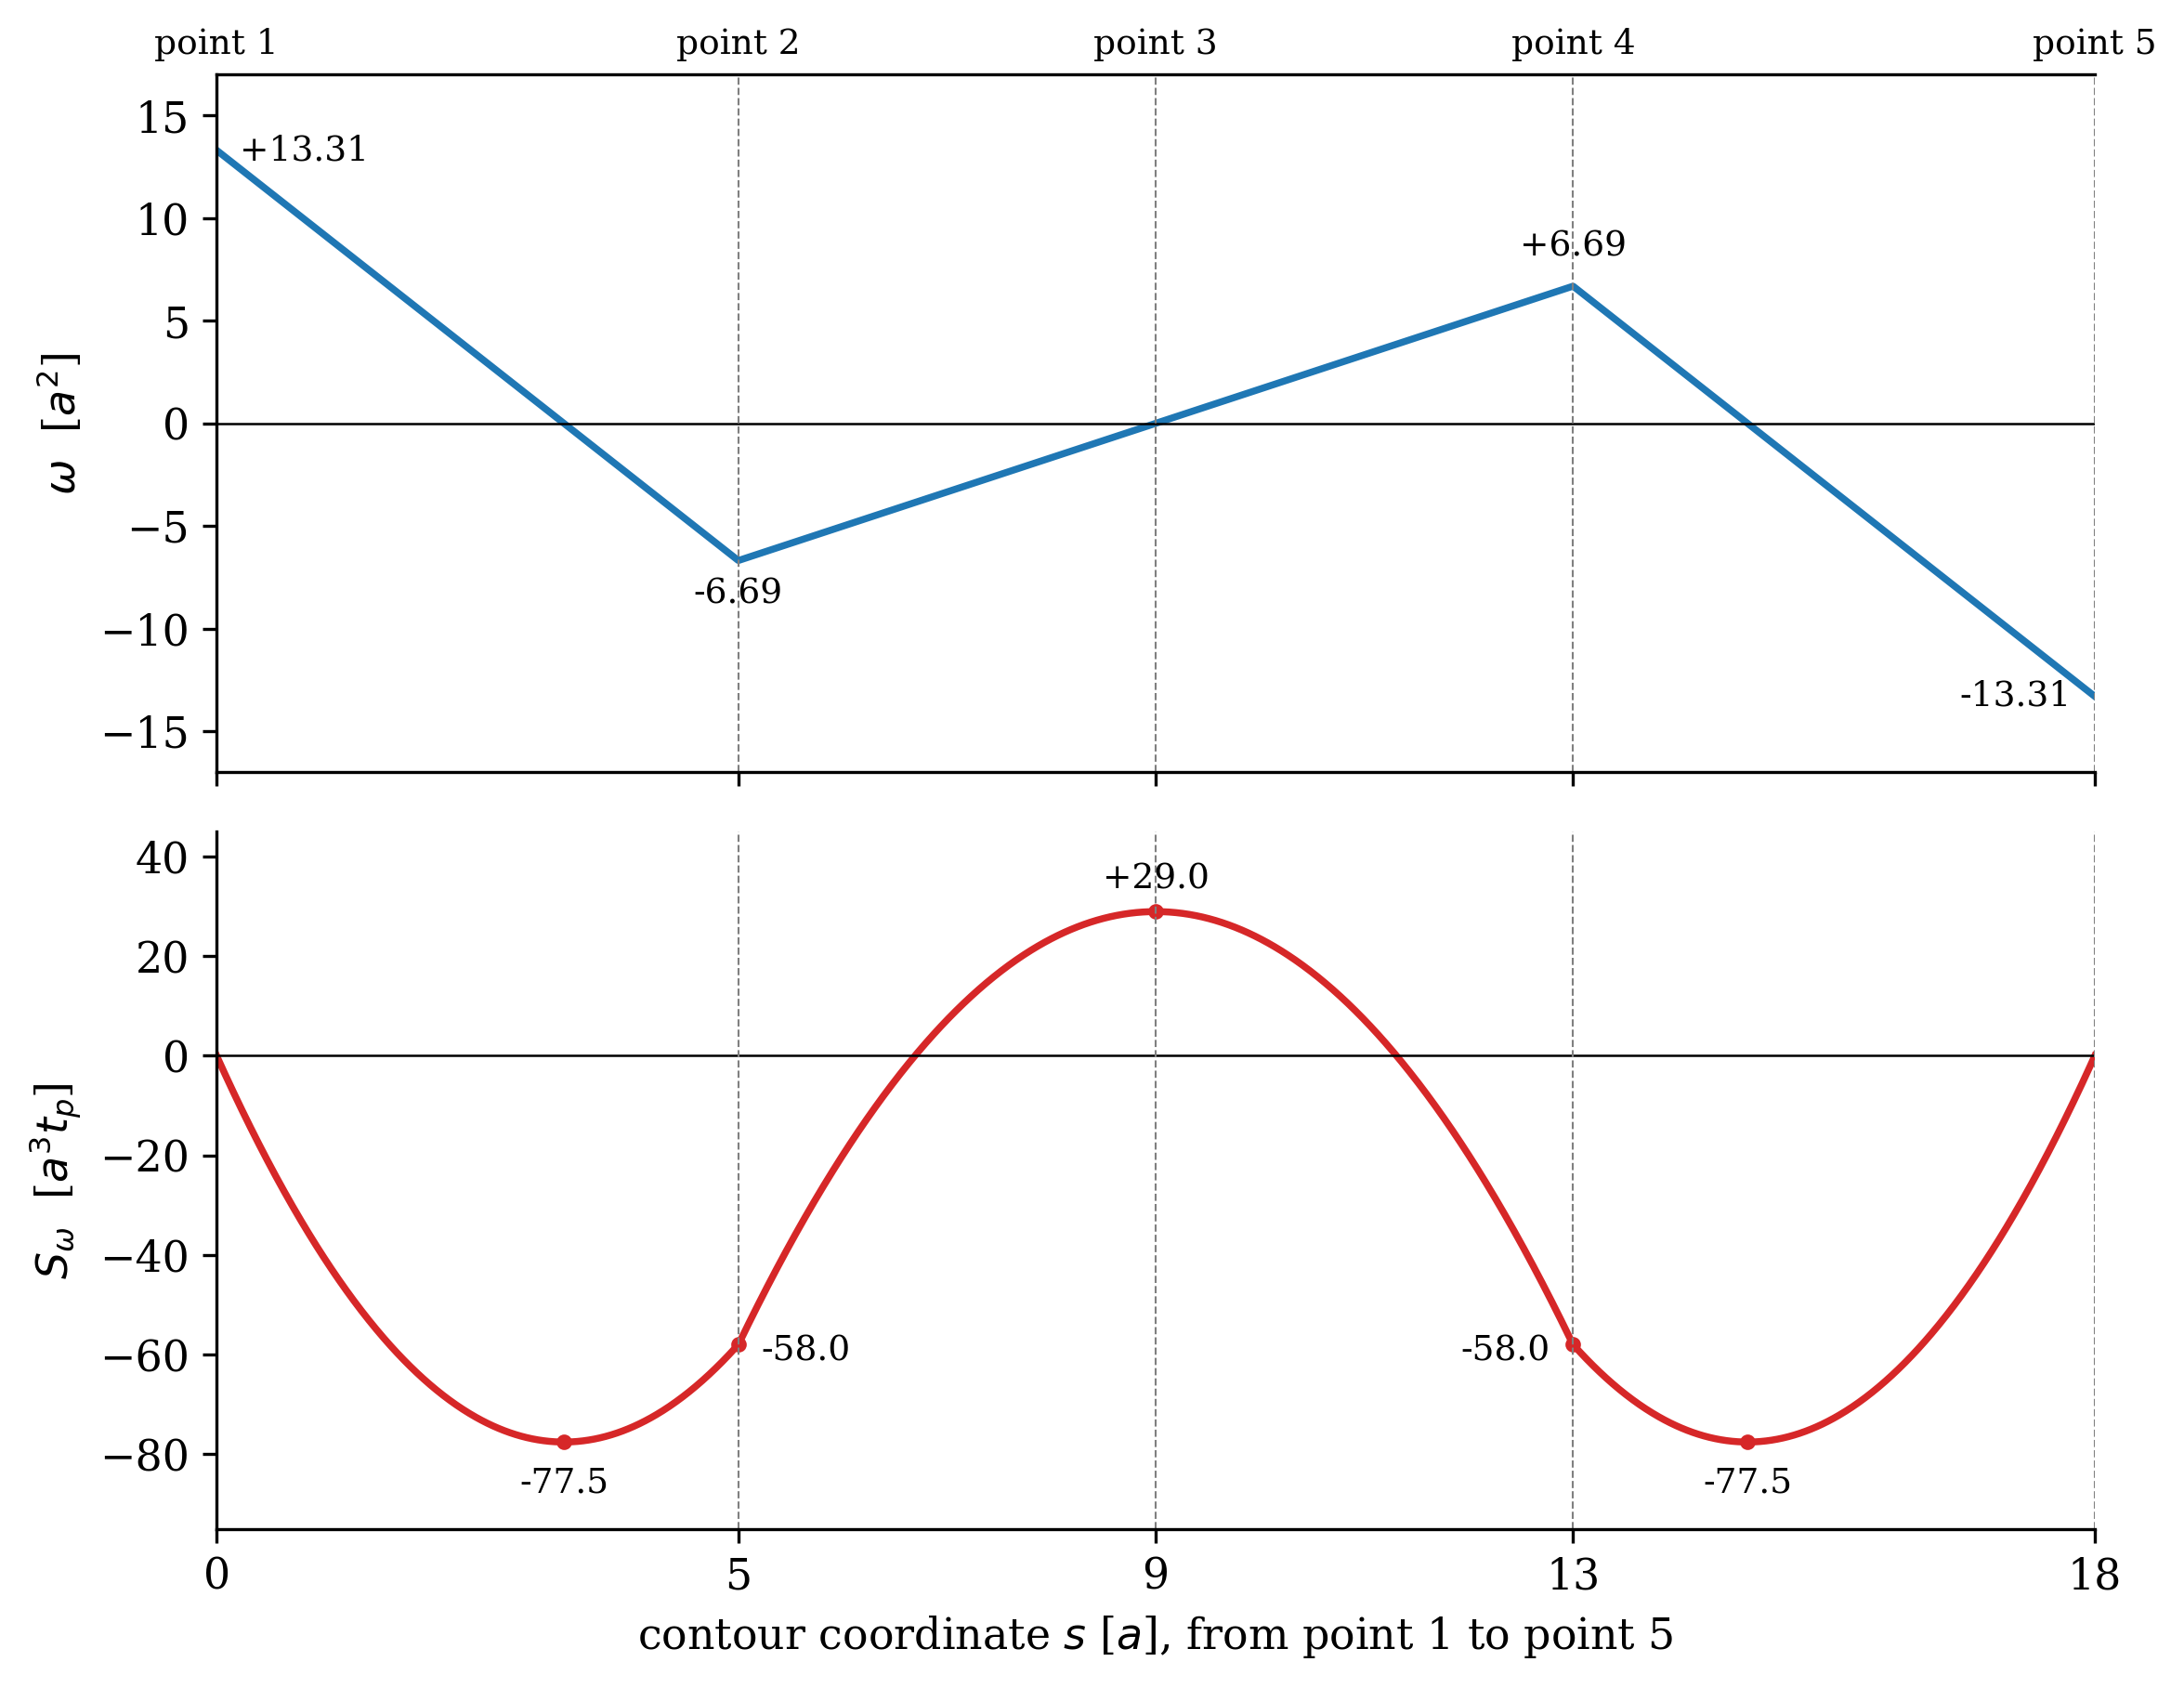
\includegraphics[width=0.85\textwidth]{figures/BU_omega_Somega_plot}
  \caption{Sectorial coordinate $\omega(s)$ (top) and sectorial area moment
    $S_\omega(s)$ (bottom) along the contour of design BU, from point 1 (top of
    the port side shell) to point 5 (top of the starboard side shell).}
  \label{fig:BU_plot}
\end{figure}

\finalanswer{$\omega$ is linear along each part: $0$ in point 3 and on the side shells at $z = e = 1.672a$, $\mp 6.69\,a^2$ in the bottom corners and $\pm 13.31\,a^2$ at the tops of the side shells, where the warping is largest. $S_\omega$ is quadratic along each part: $0$ at both free edges, $-77.5\,a^3t_p$ in the side shells at $z=e$, $-58.0\,a^3t_p$ in the corners and $+29.0\,a^3t_p$ in point 3. The warping shear stress ($\propto S_\omega/t$) is largest in the side shells at $z = e$.}


\newpage
\section{Torsion and warping constants of design BU}
\label{sec:a2-6}

\questionbox{Calculate the torsion constant $I_p(A,B,t_{bp},t_{sp})$ and warping
constant $I_w(A,B,t_{bp},t_{sp})$ for the simplified model of section BU.
Present $I_w(a,t_p)$ using $A=8a$, $B=5a$, $t_{sp}=3.5t_p$ and $t_{bp}=6.5t_p$.
\textbf{(3 pts)}}



\subsection{Torsion constant}

BU is an open thinwalled section. In the lectures we saw that for one thin plate with length $L$ and thickness $t$ the torsion constant is

\begin{equation}
  I_{p,i} = \frac{1}{3}\,L_i\,t_i^3 .
\end{equation}

An open section is just a number of these plates connected to each other, so we can add them up piecewise:

\begin{equation}
  I_p = \frac{1}{3}\sum_i L_i\,t_i^3 .
  \label{eq:a26-Ip-sum}
\end{equation}

Our U-section has one bottom plate (length $A$, thickness $t_{bp}$) and two side shells (length $B$, thickness $t_{sp}$), so

\begin{equation}
  \boxed{\;I_p(A,B,t_{bp},t_{sp}) = \frac{1}{3}\left(A\,t_{bp}^3 + 2B\,t_{sp}^3\right)\;}
  \label{eq:a26-Ip}
\end{equation}

Filling in $A=8a$, $B=5a$, $t_{bp}=6.5t_p$ and $t_{sp}=3.5t_p$ gives

\begin{align}
  I_{p,bottom} &= \tfrac{1}{3}\cdot 8a\cdot(6.5t_p)^3 = \tfrac{1}{3}\cdot 2197\,a t_p^3 = 732.3\,a t_p^3,\\
  I_{p,sides}  &= \tfrac{2}{3}\cdot 5a\cdot(3.5t_p)^3 = \tfrac{1}{3}\cdot 428.8\,a t_p^3 = 142.9\,a t_p^3,\\
  I_p &= 732.3 + 142.9 = 875\,a t_p^3 .
\end{align}

The bottom plate gives $732.3/875 = 0.84$, so 84\,\% of $I_p$, while the two side shells together are actually longer ($10a$ vs.\ $8a$). This is because the thickness is cubed, so the thicker bottom plate counts much more.

\subsection{Warping constant}

The warping constant is

\begin{equation}
  I_w = \int_A \omega^2\,\mathrm{d}A = \int_s \omega^2(s)\,t(s)\,\mathrm{d}s .
  \label{eq:a26-Iw-def}
\end{equation}

For $\omega$ we use the sectorial coordinate from Section~\ref{sec:a2-5}. It is important that this one is taken around the shear centre S, because otherwise $\omega$ also contains some bending and $I_w$ becomes too big.

The thickness is constant per plate, so we do the integral piecewise with the same parts and local $s$ as in Section~\ref{sec:a2-5}:

\begin{equation}
  I_w = \sum_i t_i \int_{s} \omega_i^2\,\mathrm{d}s .
\end{equation}

$\omega$ is antisymmetric, so $\omega^2$ is the same on both sides of the centre line. That means we only have to do the port half (parts 3--2 and 2--1)
and multiply by two.

\paragraph{Part 3--2 (bottom plate, port half).}
With $\omega_{32}(s) = -e\,s$ for $0\le s\le A/2$:

\begin{align}
  I_{w,32} &= t_{bp}\int_0^{A/2} \left(-e\,s\right)^2\mathrm{d}s
            = t_{bp}\,e^2\int_0^{A/2} s^2\,\mathrm{d}s \nonumber\\
           &= t_{bp}\,e^2\left[\frac{s^3}{3}\right]_0^{A/2}
            = \frac{t_{bp}\,e^2A^3}{24} .
\end{align}

\paragraph{Part 2--1 (port side shell).}
With $\omega_{21}(s) = \frac{A}{2}\,(s-e)$ for $0\le s\le B$:
\begin{align}
  I_{w,21} &= t_{sp}\int_0^{B} \frac{A^2}{4}\,(s-e)^2\,\mathrm{d}s
            = t_{sp}\,\frac{A^2}{4}\int_0^{B} \left(s^2 - 2e\,s + e^2\right)\mathrm{d}s \nonumber\\
           &= t_{sp}\,\frac{A^2}{4}\left[\frac{s^3}{3} - e\,s^2 + e^2 s\right]_0^{B}
            = t_{sp}\,\frac{A^2}{4}\left(\frac{B^3}{3} - e\,B^2 + e^2B\right) .
\end{align}

\paragraph{Total.}
Using the symmetry:
\begin{align}
  I_w &= 2\left\{\frac{t_{bp}\,e^2A^3}{24} + t_{sp}\,\frac{A^2}{4}\left(\frac{B^3}{3} - e\,B^2 + e^2B\right)\right\} \nonumber\\
      &= \frac{t_{bp}\,e^2A^3}{12} + t_{sp}\,\frac{A^2}{2}\left(\frac{B^3}{3} - e\,B^2 + e^2B\right),
  \label{eq:a26-Iw-e}
\end{align}
with $e = 3B^2 t_{sp}/(A t_{bp} + 6B t_{sp})$ from Section~\ref{sec:a2-5}.

\subsection{Warping constant in terms of $a$ and $t_p$}

Now we fill in $A=8a$, $B=5a$, $t_{bp}=6.5t_p$, $t_{sp}=3.5t_p$ and $e=1.672a$:
\begin{align}
  I_{w,32} &= \frac{6.5\cdot1.672^2\cdot8^3}{24}\,a^5t_p = 387.7\,a^5t_p,\\
  I_{w,21} &= 3.5\cdot\frac{8^2}{4}\left(\frac{5^3}{3} - 1.672\cdot5^2 + 1.672^2\cdot5\right)a^5t_p \nonumber\\
           &= 56\,(41.67 - 41.80 + 13.98)\,a^5t_p = 775.3\,a^5t_p,
\end{align}
so
\begin{equation}
  I_w = 2\,(387.7 + 775.3)\,a^5t_p = 2326\,a^5t_p \approx 2.33\cdot10^3\,a^5t_p .
\end{equation}
The side shells give $2\cdot775.3/2326 = 0.67$, so about two thirds of $I_w$.
That makes sense, since the warping is largest at the top of the side shells
($|\omega| = 13.31a^2$) and $\omega$ is squared.

\subsection{Closed-form expression}

Equation~\eqref{eq:a26-Iw-e} still has $e$ in it. To get $I_w$ only in $A$, $B$,
$t_{bp}$ and $t_{sp}$ we also fill in $e$. First we write everything over
$A^2/12$:
\begin{equation}
  I_w = \frac{A^2}{12}\Big[e^2\left(A t_{bp} + 6B t_{sp}\right) - 6B^2 t_{sp}\,e + 2B^3 t_{sp}\Big] .
\end{equation}
To keep it short we call $D = A t_{bp} + 6B t_{sp}$, so $e = 3B^2 t_{sp}/D$.
Then
\begin{equation}
  e^2 D = \frac{9B^4 t_{sp}^2}{D},\qquad 6B^2 t_{sp}\,e = \frac{18B^4 t_{sp}^2}{D},
\end{equation}
so the part between the brackets becomes
\begin{equation}
  -\frac{9B^4 t_{sp}^2}{D} + 2B^3 t_{sp}
  = \frac{B^3 t_{sp}\left(2D - 9B t_{sp}\right)}{D}
  = \frac{B^3 t_{sp}\left(2A t_{bp} + 3B t_{sp}\right)}{A t_{bp} + 6B t_{sp}} .
\end{equation}
and we get
\begin{equation}
  \boxed{\;I_w(A,B,t_{bp},t_{sp}) = \frac{A^2 B^3 t_{sp}\left(2A t_{bp} + 3B t_{sp}\right)}{12\left(A t_{bp} + 6B t_{sp}\right)}\;}
  \label{eq:a26-Iw}
\end{equation}
With the numbers this gives the same answer as before which is a good check:
\begin{equation}
  I_w = \frac{64\cdot125\cdot3.5\,(104+52.5)}{12\,(52+105)}\,a^5t_p
      = \frac{4\,382\,000}{1884}\,a^5t_p = 2326\,a^5t_p .
\end{equation}


\finalanswer{
\begin{align*}
  I_p(A,B,t_{bp},t_{sp}) &= \tfrac{1}{3}\left(A\,t_{bp}^3 + 2B\,t_{sp}^3\right),
  \qquad I_p(a,t_p) = 875\,a\,t_p^3,\\[4pt]
  I_w(A,B,t_{bp},t_{sp}) &= \frac{t_{bp}\,e^2A^3}{12} + t_{sp}\,\frac{A^2}{2}\left(\frac{B^3}{3} - e\,B^2 + e^2B\right)\\
  &= \frac{A^2 B^3 t_{sp}\left(2A t_{bp} + 3B t_{sp}\right)}{12\left(A t_{bp} + 6B t_{sp}\right)},\\[4pt]
  I_w(a,t_p) &= 2.33\cdot10^3\,a^5 t_p .
\end{align*}}





\newpage
\section{Effect of closing the hatch cover}
\label{sec:a2-7}

\questionbox{For the simple geometry, consider the hatch cover both open (BU)
and closed (BUH). What is the improvement in $I_p(a,t_p)$ when closing the hatch
cover? The thickness of the hatch cover is $t_{hp}=2.5t_p$; Bredt's thin-walled
theory is assumed for the closed section. \textbf{(4 pts)}}



When the hatch cover is closed, the U-section becomes a single closed cell (design BUH), see Figure~\ref{fig:BUH_section}. The bottom plate and side shells stay the same as in BU, and on top we now have the hatch cover with thickness $t_{hp} = 2.5t_p$.

\begin{figure}[h]
    \centering
    \begin{tikzpicture}[scale=0.6, >={Stealth[length=2mm,width=1.6mm]},
        dim/.style={thin, {Latex[length=1.6mm,width=1.2mm]}-{Latex[length=1.6mm,width=1.2mm]}},
        ext/.style={very thin, gray}]
        % enclosed area
        \fill[blue!8] (-4,0) rectangle (4,5);
        \node at (0,3.3) {$\Omega = A\cdot B$};
        % plates (line width ~ thickness)
        \draw[line width=2.6pt, line cap=rect] (-4,0) -- (4,0);   % bottom
        \draw[line width=1.4pt] (-4,0) -- (-4,5);                 % port side
        \draw[line width=1.4pt] ( 4,0) -- ( 4,5);                 % stb side
        \draw[line width=1.0pt, line cap=rect] (-4,5) -- (4,5);   % hatch cover
        % shear flow (counter-clockwise)
        \draw[->, red!75!black, thick] (-1.2,1.1) -- (1.2,1.1);
        \draw[->, red!75!black, thick] (3.2,1.2) -- (3.2,3.8);
        \draw[->, red!75!black, thick] (1.2,3.9) -- (-1.2,3.9);
        \draw[->, red!75!black, thick] (-3.2,3.8) -- (-3.2,1.2);
        \node[red!75!black] at (0,1.6) {$q$};
        % labels
        \node[above, font=\small] at (0,5.05) {$t_{hp}$};
        \node[below, font=\small] at (0,-0.1) {$t_{bp}$};
        \node[left,  font=\small] at (-4.1,2.5) {$t_{sp}$};
        \node[right, font=\small] at ( 4.1,2.5) {$t_{sp}$};
        % dimensions
        \foreach \x in {-4,4} \draw[ext] (\x,-0.2) -- (\x,-1.45);
        \draw[dim] (-4,-1.3) -- node[below, font=\small] {$A = 8a$} (4,-1.3);
        \foreach \y in {0,5} \draw[ext] (4.2,\y) -- (5.95,\y);
        \draw[dim] (5.8,0) -- node[right, font=\small] {$B = 5a$} (5.8,5);
    \end{tikzpicture}
    \caption{Design BUH: the U-section with a closed hatch cover forms one closed
             cell with enclosed area $\Omega$ and a constant shear flow $q$.}
    \label{fig:BUH_section}
\end{figure}

\subsection{Torsion constant of the closed section (Bredt)}

For a thin-walled closed section we use Bredt's theory. In the lectures the
torsion constant of a single cell follows from the 2nd Bredt formula:
\begin{equation}
  I_p = \frac{4\,\Omega^2}{\displaystyle\oint_s \frac{1}{t_p(s)}\,\mathrm{d}s} ,
  \label{eq:a27-bredt}
\end{equation}
where $\Omega$ is the area enclosed by the centre line of the walls.

\paragraph{Enclosed area.}
The cell is a rectangle of $A$ by $B$:
\begin{equation}
  \Omega = A\,B = 8a\cdot5a = 40\,a^2 .
\end{equation}

\paragraph{Contour integral.}
The thickness is constant per plate, so the contour integral is again done piecewise, now over all four walls of the cell:
\begin{equation}
  \oint_s \frac{1}{t_p(s)}\,\mathrm{d}s
  = \frac{A}{t_{bp}} + \frac{2B}{t_{sp}} + \frac{A}{t_{hp}} .
\end{equation}
With the numbers:
\begin{align}
  \oint_s \frac{1}{t_p(s)}\,\mathrm{d}s
  &= \left(\frac{8}{6.5} + \frac{2\cdot5}{3.5} + \frac{8}{2.5}\right)\frac{a}{t_p} \nonumber\\
  &= \left(1.231 + 2.857 + 3.200\right)\frac{a}{t_p} = 7.288\,\frac{a}{t_p} .
\end{align}
The hatch cover gives the largest term: it is as long as the bottom plate but much thinner.

\paragraph{Torsion constant.}
Putting this in Equation~\eqref{eq:a27-bredt}:
\begin{equation}
  I_{p,BUH}(A,B,t_{bp},t_{sp},t_{hp})
  = \frac{4A^2B^2}{\dfrac{A}{t_{bp}} + \dfrac{2B}{t_{sp}} + \dfrac{A}{t_{hp}}} ,
\end{equation}
\begin{equation}
  I_{p,BUH} = \frac{4\cdot(40a^2)^2}{7.288\,a/t_p}
            = \frac{6400}{7.288}\,a^3t_p = 878\,a^3t_p .
\end{equation}

\subsection{Improvement compared to the open section}

From Section~\ref{sec:a2-6} the open section has $I_{p,BU} = 875\,a\,t_p^3$.
The ratio between the two is
\begin{equation}
  \frac{I_{p,BUH}}{I_{p,BU}} = \frac{878\,a^3t_p}{875\,a\,t_p^3}
  = 1.00\left(\frac{a}{t_p}\right)^2 .
\end{equation}
So closing the hatch cover increases $I_p$ by a factor $(a/t_p)^2$. Since $t_p$ is much smaller than $a$ this is a very large number. For example, with $a = 1$\,m and $t_p = 10$\,mm we get $a/t_p = 100$, so the section becomes about $10^4$ times stiffer in torsion. This is the same kind of result as the open and closed circular section from the lectures, where the closed one also came out a factor $3\,(r/t_p)^2$ stiffer.

\paragraph{Why the difference is so big.}
In the open section BU the shear stresses can only go up and down within the thickness of each plate, so the lever arm is of the order of $t_p$. That is why $I_{p,BU}$ scales with $t_p^3$. In the closed section the shear flow $q$ goes around the whole cell, so the lever arm is of the order of the size of the cell ($a$). That is why $I_{p,BUH}$ scales with $\Omega^2 t_p$, so with $a^3 t_p$.


\finalanswer{
With the hatch cover closed the section is one closed cell, and Bredt gives
\[
  I_{p,BUH} = \frac{4A^2B^2}{\dfrac{A}{t_{bp}} + \dfrac{2B}{t_{sp}} + \dfrac{A}{t_{hp}}}
  = 878\,a^3t_p ,
\]
compared to $I_{p,BU} = 875\,a\,t_p^3$ for the open section. The improvement is
\[
  \frac{I_{p,BUH}}{I_{p,BU}} = 1.00\left(\frac{a}{t_p}\right)^2 ,
\]
so about $10^4$ for $a/t_p = 100$.}
